\documentclass[11pt]{article}

\usepackage[letterpaper]{geometry}
%\usepackage[letterpaper,left=2.5cm,top=2cm,right=2.5cm,bottom=2cm]{geometry}

\usepackage[utf8]{inputenc}
\usepackage{mathpazo}
\usepackage{amsmath}
\usepackage{amsfonts}
\usepackage{siunitx}
\usepackage{cancel}

\usepackage{graphicx}
\usepackage{float}
\usepackage{empheq}
\usepackage[most]{tcolorbox}

\newtcbox{\mymath}[1][]{%
  nobeforeafter, math upper, tcbox raise base,
  enhanced, colframe=black!30!black,
  colback=yellow!30, boxrule=1pt,
  #1}

% Hyperlinks with decent looking default colors.
\usepackage{hyperref}
\usepackage{xcolor}
\hypersetup{
  colorlinks,
  linkcolor={red!50!black},
  citecolor={blue!50!black},
  urlcolor={blue!80!black}
}

% For those sexy spaced low small caps from classic-thesis!
\usepackage{microtype}
\usepackage{textcase}
\DeclareRobustCommand{\spacedlowsmallcaps}[1]{%
  \textls[80]{\scshape\MakeTextLowercase{#1}}%
}

% Replaced mathpazo \sum symbol with computer modern's.
\DeclareSymbolFont{cmlargesymbols}{OMX}{cmex}{m}{n}
\let\sumop\relax
\DeclareMathSymbol{\sumop}{\mathop}{cmlargesymbols}{"50}

\newcommand{\forceindent}{\leavevmode{\parindent=1em\indent}}

\usepackage{fancyhdr}
\pagestyle{fancy} 
\fancyhead{}
\rhead{Ali Ramadhan}
\lhead{6.339 Project 2---Finite Volume Methods}
\cfoot{\thepage}

\title{\spacedlowsmallcaps{6.339: Numerical Methods for Partial Differential Equations}\\ \spacedlowsmallcaps{Project two: Finite Volume Methods}}
\author{Ali Ramadhan$^\text{†}$ (\texttt{alir@mit.edu})}
\date{\textit{$^\text{†}$Department of Earth, Atmospheric, and Planetary Sciences}}

\renewcommand\thesubsection{\thesection(\alph{subsection})}

\begin{document}
\maketitle

In this project, we will utilize finite volume methods to study dense traffic flow and traffic jams modeled as shockwaves. We model traffic in each lane by a scalar hyperbolic conservation law, following what is known as the Lighthill-Whitman-Richards model.

We use a scalar hyperbolic conservation law to model traffic density $\rho^{(\ell)}(x,t)$ for $n$ lanes indexed by $\ell = 1,2,\dots,n$
\begin{equation} \label{eq:conservationLaw}
	\frac{\partial \rho^{(\ell)}}{\partial t} + \frac{\partial (\rho^{(\ell)} v^{(\ell)})}{\partial x} = s^{(\ell)}
\end{equation}
where $v^{(\ell)}(x,t)$ is the average velocity of the cars in lane $\ell$. This, however, provides us with only one equation for two unknowns and thus we specify the velocity by
\begin{equation} \label{eq:velocity}
	v^{(\ell)}(\rho^{(\ell)}) = v_\mathrm{max} \left( 1 - \frac{\left(\rho^{(\ell)}\right)^2}{\rho_\mathrm{max}^2} \right)
\end{equation}
where $\rho_\mathrm{max}$ and $v_\mathrm{max}$ are the lane-independent maximum traffic density and velocity respectively. This gives us a traffic flux of 
\begin{equation} \label{eq:flux}
f^{(\ell)}(\rho^{(\ell)}) = \rho^{(\ell)} v^{(\ell)} = v_\mathrm{max} \left( \rho^{(\ell)} - \frac{\left(\rho^{(\ell)}\right)^3}{\rho_\mathrm{max}^2} \right)
\end{equation}
The source term
\begin{equation} \label{eq:source}
	s^{(\ell)} = \sumop_{\substack{|k-\ell|=1 \\ 1 \le k,\ell \le n}} \alpha \left( \rho^{(k)} - \rho^{(\ell)} \right)
\end{equation}
models the density of traffic that is switching into lane $\ell$ from neighboring lanes. $\alpha$ is the fraction of drivers that change lanes.

\section{Solution by a first-order finite volume scheme}

We will split up our one-dimensional grid into a number of cells indexed by $i=1,2,\ldots,N$. We will index the edges of the cell $i$ by $i-\frac{1}{2}$ for the left boundary of the cell, and by $i+\frac{1}{2}$ for the right boundary of the cell. So we can think of $i$ as indexing the cell centers.

To derive a first-order conservative finite-volume scheme for a single lane, we will consider the volume averages of the traffic density $\rho(x,t)$ at two different times. The volume average of the traffic density at cell $i$, $\rho_i = \rho(x_i,t)$, at a time $t_1$ over $x \in \left[ x_{i-\frac{1}{2}}, x_{i+\frac{1}{2}} \right]$ must exist by the mean value theorem and is given by
\begin{equation*}
	\bar{\rho}_i(t_1) = \frac{1}{\Delta x_i} \int_{x_{i-\frac{1}{2}}}^{x_{i+\frac{1}{2}}} \rho(x,t_1) \; dx
\end{equation*}
and an identical expression can be written for the volume average at a later time $t_2 > t_1$. Now, integrating the scalar conservation law in time from $t = t_1$ to $t = t_2$ we can write
\begin{equation*}
	\int_{t_1}^{t_2} \frac{\partial\bar{\rho}}{\partial t} \; dt + \int_{t_1}^{t_2} \frac{\partial(\bar{\rho} v)}{\partial x} \; dt = 0
\end{equation*}                         
where the first integral can be evaluated using the second fundamental theorem of calculus, sometimes referred to as the Newton–Leibniz axiom, and rearranged to obtain $\bar{\rho}_i$ at a later time
\begin{equation*}
\bar{\rho}(x,t_2) = \bar{\rho}(x,t_1) - \int_{t_1}^{t_2} \frac{\partial(\bar{\rho}_i v_i)}{\partial x} \; dt
\end{equation*}

We can now calculate $\rho_i(t_2)$ as
\begin{align*}
\bar{\rho}_i(t_2) &=
	\frac{1}{\Delta x_i} \int_{x_{i-\frac{1}{2}}}^{x_{i+\frac{1}{2}}} \left[ \rho(x,t_1) - \int_{t_1}^{t_2} \frac{\partial(\rho v)}{\partial x} \; dt \right] \; dx \\
	&= \frac{1}{\Delta x_i} \int_{x_{i-\frac{1}{2}}}^{x_{i+\frac{1}{2}}} \rho(x,t_1) \; dx - \frac{1}{\Delta x_i} \int_{x_{i-\frac{1}{2}}}^{x_{i+\frac{1}{2}}} \int_{t_1}^{t_2} \frac{\partial(\rho v)}{\partial x} \; dt \; dx \\
	&= \bar{\rho}_i(t_1) - \frac{1}{\Delta x_i} \int_{t_1}^{t_2} \left[ \rho(x_{i+\frac{1}{2}}, t) v(x_{i+\frac{1}{2}}, t) - \rho(x_{i-\frac{1}{2}}, t) v(x_{i-\frac{1}{2}}, t) \right] \; dt \\
	&= \bar{\rho}_i(t_1) - \frac{1}{\Delta x_i} \left[ \int_{t_1}^{t_2} F_{i+\frac{1}{2}} - F_{i-\frac{1}{2}} \right] \; dt
\end{align*}
which can be rearranged to write
\begin{equation*}
	\bar{\rho}_i(t_2) - \bar{\rho}_i(t_1) = \frac{d}{dt} \int_{t_1}^{t_2} \rho_i(t) \; dt = \int_{t_1}^{t_2} \left( - \frac{F_{i+\frac{1}{2}} - F_{i-\frac{1}{2}}}{\Delta x_i} \right) \; dt
\end{equation*}
where the integrands inside the two integrals must be the same so that
\begin{equation*} \label{eq:drhodt}
	\frac{d \bar{\rho}_i}{dt} = - \frac{F_{i+\frac{1}{2}} - F_{i-\frac{1}{2}}}{\Delta x_i}
\end{equation*}
and if we approximate the time derivate by a first-order forward difference finite difference operator $\dot{\bar{\rho}}_i = (\bar{\rho}_i^{n+1} - \bar{\rho}_i^n)/\Delta t$ and further rearrange, we obtain
\begin{equation} \label{eq:firstorder}
	\bar{\rho}_i^{n+1} = \bar{\rho}_i^n - \frac{\Delta t}{\Delta x_i} \left( F_{i+\frac{1}{2}} - F_{i-\frac{1}{2}} \right) 
\end{equation}

\subsection{Solving the Riemann problem for Gudonov's scheme}
\begin{tcolorbox}
  \textit{Analyzing $f(\rho)$ determine the Godunov scheme flux in a manner that does not require a brute force search for the minimum/maximum of the flux between $\rho_i$ and $\rho_{i+1}$.}
\end{tcolorbox}

For the Gudonov scheme we will show that we can solve the Riemann problem exactly and without the use of a brute force search. We first notice that the flux function \eqref{eq:flux} is a cubic function, increasing monotonically until it attains a maximum value of $\rho_\mathrm{max}/\sqrt{3}$ and then decreases monotonically. The maximum was found by setting the derivative of \eqref{eq:flux} to zero and solving for the value of $\rho$ that maximizes $f(\rho)$:
\begin{equation*}
  \frac{df}{d\rho} = v_\mathrm{max} \left( 1 - \frac{3\rho^2}{\rho_\mathrm{max}^2} \right) = 0 \quad \implies \quad \rho = \frac{\rho_\mathrm{max}}{\sqrt{3}}
\end{equation*}

Focusing on the case when $\rho_i < \rho_{i+1}$ first, we are interested in finding the minimum of $f(\rho)$ over the interval $[\rho_i, \rho_{i+1}]$. If $\rho_i < \rho_{i+1} \le \rho_\mathrm{max}/\sqrt{3}$ then the minimum must be attained on the left endpoint, and is $f(\rho_i)$. On the other side of the maximum, if $\rho_\mathrm{max}/\sqrt{3} \le \rho_i < \rho_{i+1}$, then the minimum must be attained on the right endpoint, and is $f(\rho_{i+1})$. If the interval contains the maximum within it, then the minimum must be attained at one of the endpoints, and both must be checked. Thus we can analytically evaluate the minimum as
\begin{equation} \label{eq:min_f}
\min_{\rho \in \left[\rho_i, \rho_{i+1}\right]} f(\rho) =
\begin{cases}
  f(\rho_i),&
    \text{if } \rho_i < \rho_{i+1} \le \frac{\rho_\mathrm{max}}{\sqrt{3}} \\
  f(\rho_{i+1}),&
    \text{if } \frac{\rho_\mathrm{max}}{\sqrt{3}} \le \rho_i < \rho_{i+1} \\
  \min\left\{ f(\rho_i), f(\rho_{i+1}) \right\} ,&
    \text{if } \rho_i < \frac{\rho_\mathrm{max}}{\sqrt{3}} < \rho_{i+1}
\end{cases}
\end{equation}
The maximum can be evaluated analytically following a very similar argument for the case when $\rho_{i+1} < \rho_i$.  If $\rho_{i+1} < \rho_i \le \rho_\mathrm{max}/\sqrt{3}$ then the maximum must be attained on the right endpoint, and is $f(\rho_i)$. If $\rho_\mathrm{max}/\sqrt{3} \le \rho_{i+1} < \rho_i$, then the maximum must be attained on the left endpoint, and is $f(\rho_{i+1})$. If the interval contains the maximum within it, then we simply evaluate $f(\rho_\mathrm{max}/\sqrt{3})$ to obtain the global maximum. All together, the maximum can be expressed analytically as
\begin{equation} \label{eq:max_f}
\max_{\rho \in \left[\rho_i, \rho_{i+1}\right]} f(\rho) =
\begin{cases}
  f(\rho_i),&
    \text{if } \rho_{i+1} < \rho_i \le \frac{\rho_\mathrm{max}}{\sqrt{3}} \\
  f(\rho_{i+1}),&
    \text{if } \frac{\rho_\mathrm{max}}{\sqrt{3}} \le \rho_{i+1} < \rho_i \\
  f\left( \frac{\rho_\mathrm{max}}{\sqrt{3}} \right) ,&
  \text{if } \rho_{i+1} < \frac{\rho_\mathrm{max}}{\sqrt{3}} < \rho_i
\end{cases}
\end{equation}

\subsection{Simulating an accident for light and heavy traffic flow}
\begin{tcolorbox}
  \textit{Solve the PDE from $t = 0$ to $t = 2$. When are the specified boundary conditions not applicable? Why? How do you modify the set of boundary conditions? In what conditions can we prescribe a density on the left side of the boundary? In what conditions can we prescribe a density on the right side of the boundary? Why? Describe what happens to $\rho$ and $v$ as time evolves due to the blockage. For the traffic jam conditions, how is this related to the domino effect?}
\end{tcolorbox}

Now that we have solved the Riemann problem exactly, we can implement Gudonov's scheme using \eqref{eq:min_f} and \eqref{eq:max_f} to calculate the flux terms in \eqref{eq:firstorder} and solve for the traffic density $\rho$ as a function of time for the case of a single-lane accident as described in the problem set.

Figure \ref{fig:1b_heavy_surf} shows a heatmap of the traffic density as it evolves in time for the case of a lane initialized with heavy traffic, represented by the initial condition $\rho(0,t) = 0.8\rho_\mathrm{max}$, while figure \ref{fig:1b_light_surf} shows a heatmap of the traffic density for a lane initialized with light traffic, represented by the initial condition $\rho(0,t) = 0.2\rho_\mathrm{max}$.

\begin{figure}[h!]
  \centering
  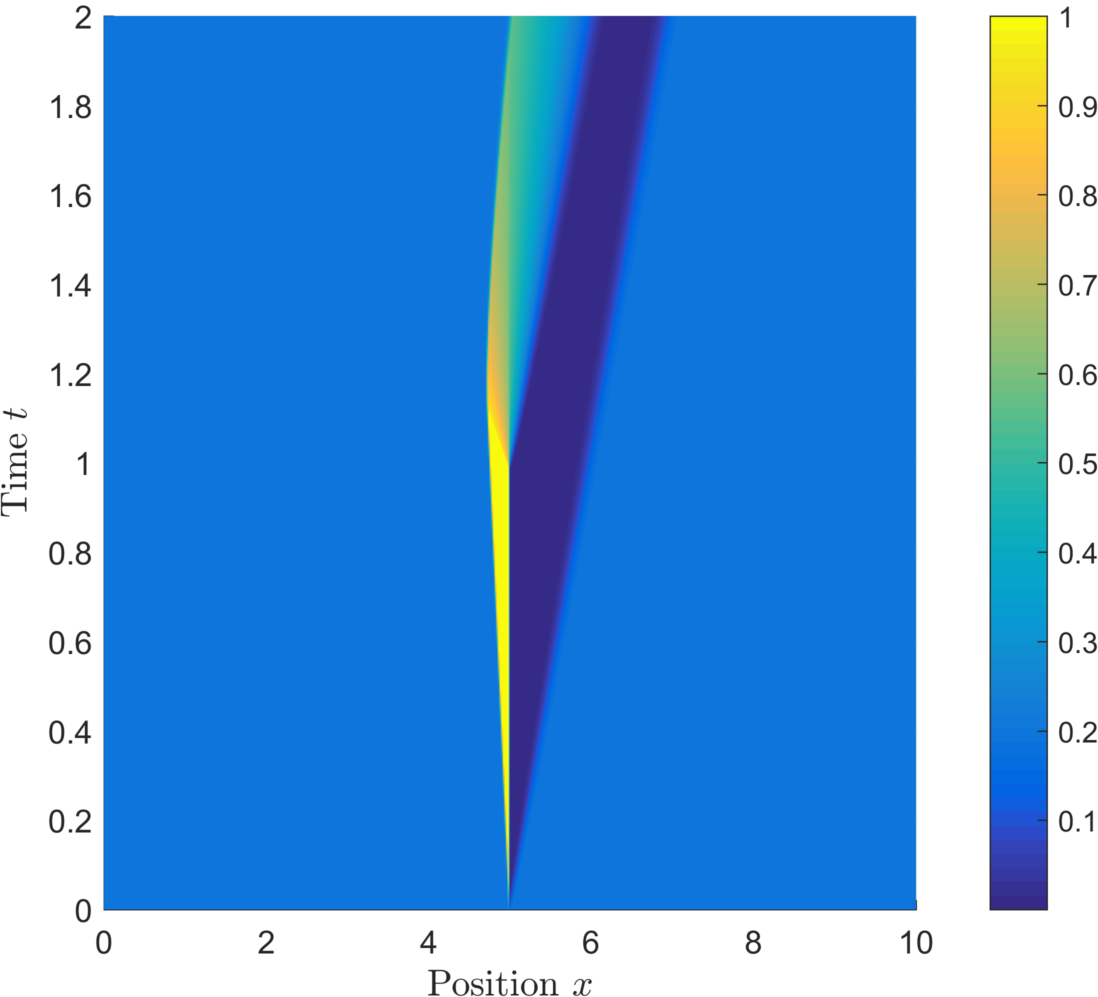
\includegraphics[width=0.75\textwidth]{1b_light_surf.png}
  \caption{Heatmap of $\rho(x,t)$ for light traffic: $\rho(0,t) = 0.2\rho_\mathrm{max}$.}
  \label{fig:1b_light_surf}
\end{figure}

\begin{figure}[h!]
  \centering
  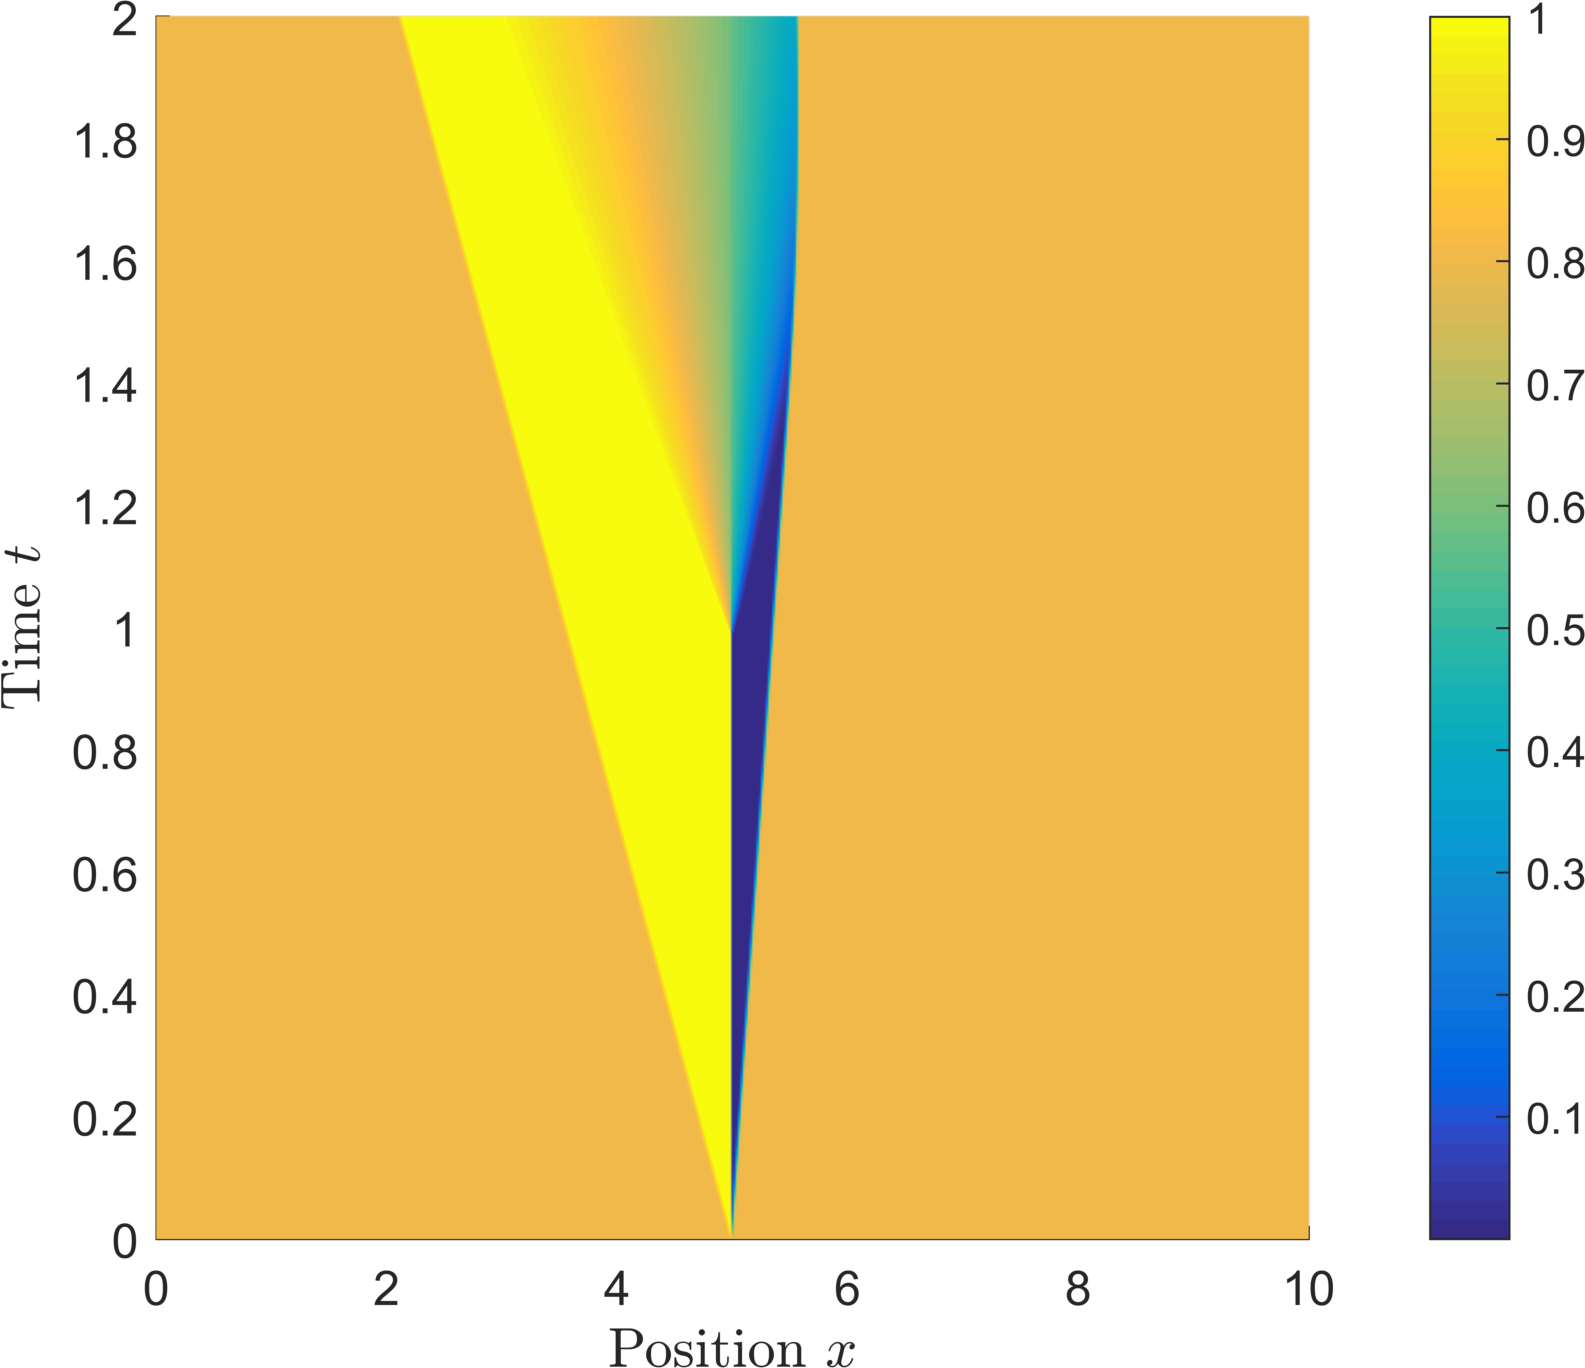
\includegraphics[width=0.75\textwidth]{1b_heavy_surf.png}
  \caption{Heatmap of $\rho(x,t)$ for heavy traffic: $\rho(0,t) = 0.8\rho_\mathrm{max}$.}
  \label{fig:1b_heavy_surf}
\end{figure}

The given boundary conditions, $\rho(0, t) = \rho_0$ and $\rho(10, t) = \rho_0$, represent Dirchlet boundary conditions specify the traffic density at the left and right boundaries. The left boundary condition can always be specified in this way as it simply represents a constant flux of cars through the $x=0$ boundary and into the single lane. However, the right boundary condition at $x=10$ cannot always be specified in this manner as it will not always make physical sense or preserve the conservation law. It also represents a constant flux of cars through the right boundary, which makes sense in the case that traffic is flowing smoothly through the single lane, but if some nonlinear behavior was to occur between the two boundaries, such as an accident or a slow driver then nothing guarantees that the flux through $x=10$ would remain at its initial value.

A problem may arise if a shockwave or traffic density wave propagates backwards towards $x=0$ at which point the constant $\rho$ boundary condition would distory the wave or shockwave. To solve this, we must employ a large enough domain such that waves do not get too close to the boundaries or stop integrating in time once the wave gets close to the boundary. In this problem set, I did not observe any waves getting close to the $x=0$ for $t \le 2$ but they do pass through the $x=10$ boundary often.

In my case, I argue that it makes sense to impose a constant boundary condition on the left $x=0$ boundary to ensure a constant influx of cars, and no boundary condition on the right (or a Neumann boundary condition of $d\rho(x=10,t)/dt=0$) to let waves propagate to the right past the boundary where they won't affect the solution on $0 \le x \le 10$. But we cannot let waves simply propagate left through the $x=0$ boundary as they should be affecting our solution with cars moving to the right---it would violate causality.

In both light and heavy traffic, we notice a stationary shockwave forms at $x=5$, the location of the accident, at $t=0$ and fans out at $t=1$ when the accident is cleared. The difference between the two is in the direction of propagation of the traffic density disturbance.

In light traffic (figure \ref{fig:1b_light_surf}) the traffic jam is small enough that every car can almost immediately start driving at the maximum speed and incoming cars do not have to stop. Bumper-to-bumper traffic is no longer the case, and a region of high (but not saturated) traffic density forms and propagates forward. The traffic density diffuses more quickly and the cars make it further than in the heavy traffic case as they can drive at a faster speed, even when catching up with the other cars that were not stopped by the accident.

In heavy traffic (figure \ref{fig:1b_heavy_surf}) the bumper-to-bumper traffic jam is sustained long after the accident is cleared. The traffic jam is long enough that not every car can begin to move. This causes a further disturbance as the dense incoming traffic must stop until all the cars in front of them have moved. The result is a traffic density disturbance, almost like a wave, representing bumper-to-bumper traffic that propagates backwards and could take a while to fully diffuse. While the cars at the front of the traffic jam can immediately start driving at full speed again, they run into the dense traffic ahead of them rather quickly which forces them to slow down. This prevents the traffic jam from diffusing quickly. Thus, even though the accident blocked the lane for 1 unit of time, the resulting traffic jam may last much longer than that and propagate a substaintial distance backwards.

The domino effect can be seen in the dynamics of heavy traffic flow. Once a few cars have to stop, the all the incoming traffic behind them must stop one by one, like a series of dominos toppling down except that new dominos keep getting added.

\section{Solution by a second-order finite volume scheme}
We will now use use a second-order scheme in which the interface values are found using the so-called limited $\kappa$-reconstructions
\begin{align}
  \rho_{i+\frac{1}{2}}^- &= \rho_i
    + \frac{1-\kappa}{4} \phi(R_i) (\rho_i - \rho_{i-1})
    + \frac{1+\kappa}{4} \phi\left(\frac{1}{R_i}\right)(\rho_{i+1} - \rho_i) \label{eq:kappa1} \\
  \rho_{i-\frac{1}{2}}^+ &= \rho_i
    - \frac{1-\kappa}{4} \phi\left(\frac{1}{R_i}\right) (\rho_{i+1} - \rho_i)
    +- \frac{1+\kappa}{4} \phi(R_i) (\rho_i - \rho_{i-1}) \label{eq:kappa2}
\end{align}
where $\displaystyle R_i = \frac{\rho_{i+1} - \rho_i}{\rho_i - \rho_{i-1}}$ is the ratio of successive slopes for the solution, $\phi(r)$ is the flux limiter function, and $\kappa$ determines the slope reconstruction scheme used. These interface values as can be plugged into the Gudonov scheme to obtain a second-order accurate flux reconstruction.

\subsection{Flux reconstruction with no limiter function}
\begin{tcolorbox}
  \textit{Using the same mesh size and time step, solve the previous traffic flow problems with the second order algorithm without limiting (i.e. set $\phi = 1$) for $\kappa = -1$, 0, and $1/3$. Describe the quality of these solutions. In particular, describe the presence of oscillations. You can for instance look at the solution at time $t = 2$.}
\end{tcolorbox}

If we use no flux limiter function, then we will set $\phi(r) = 1$ for all $r$ in the equations for the interface values \eqref{eq:kappa1} and \eqref{eq:kappa2}. Figure \ref{fig:2a_light} shows the traffic density at $t=2$ for the light traffic case using flux reconstructions with different values of $\kappa$ while figure \ref{fig:2a_heavy} shows the same for the heavy traffic case.

\begin{figure}[h!]
  \centering
  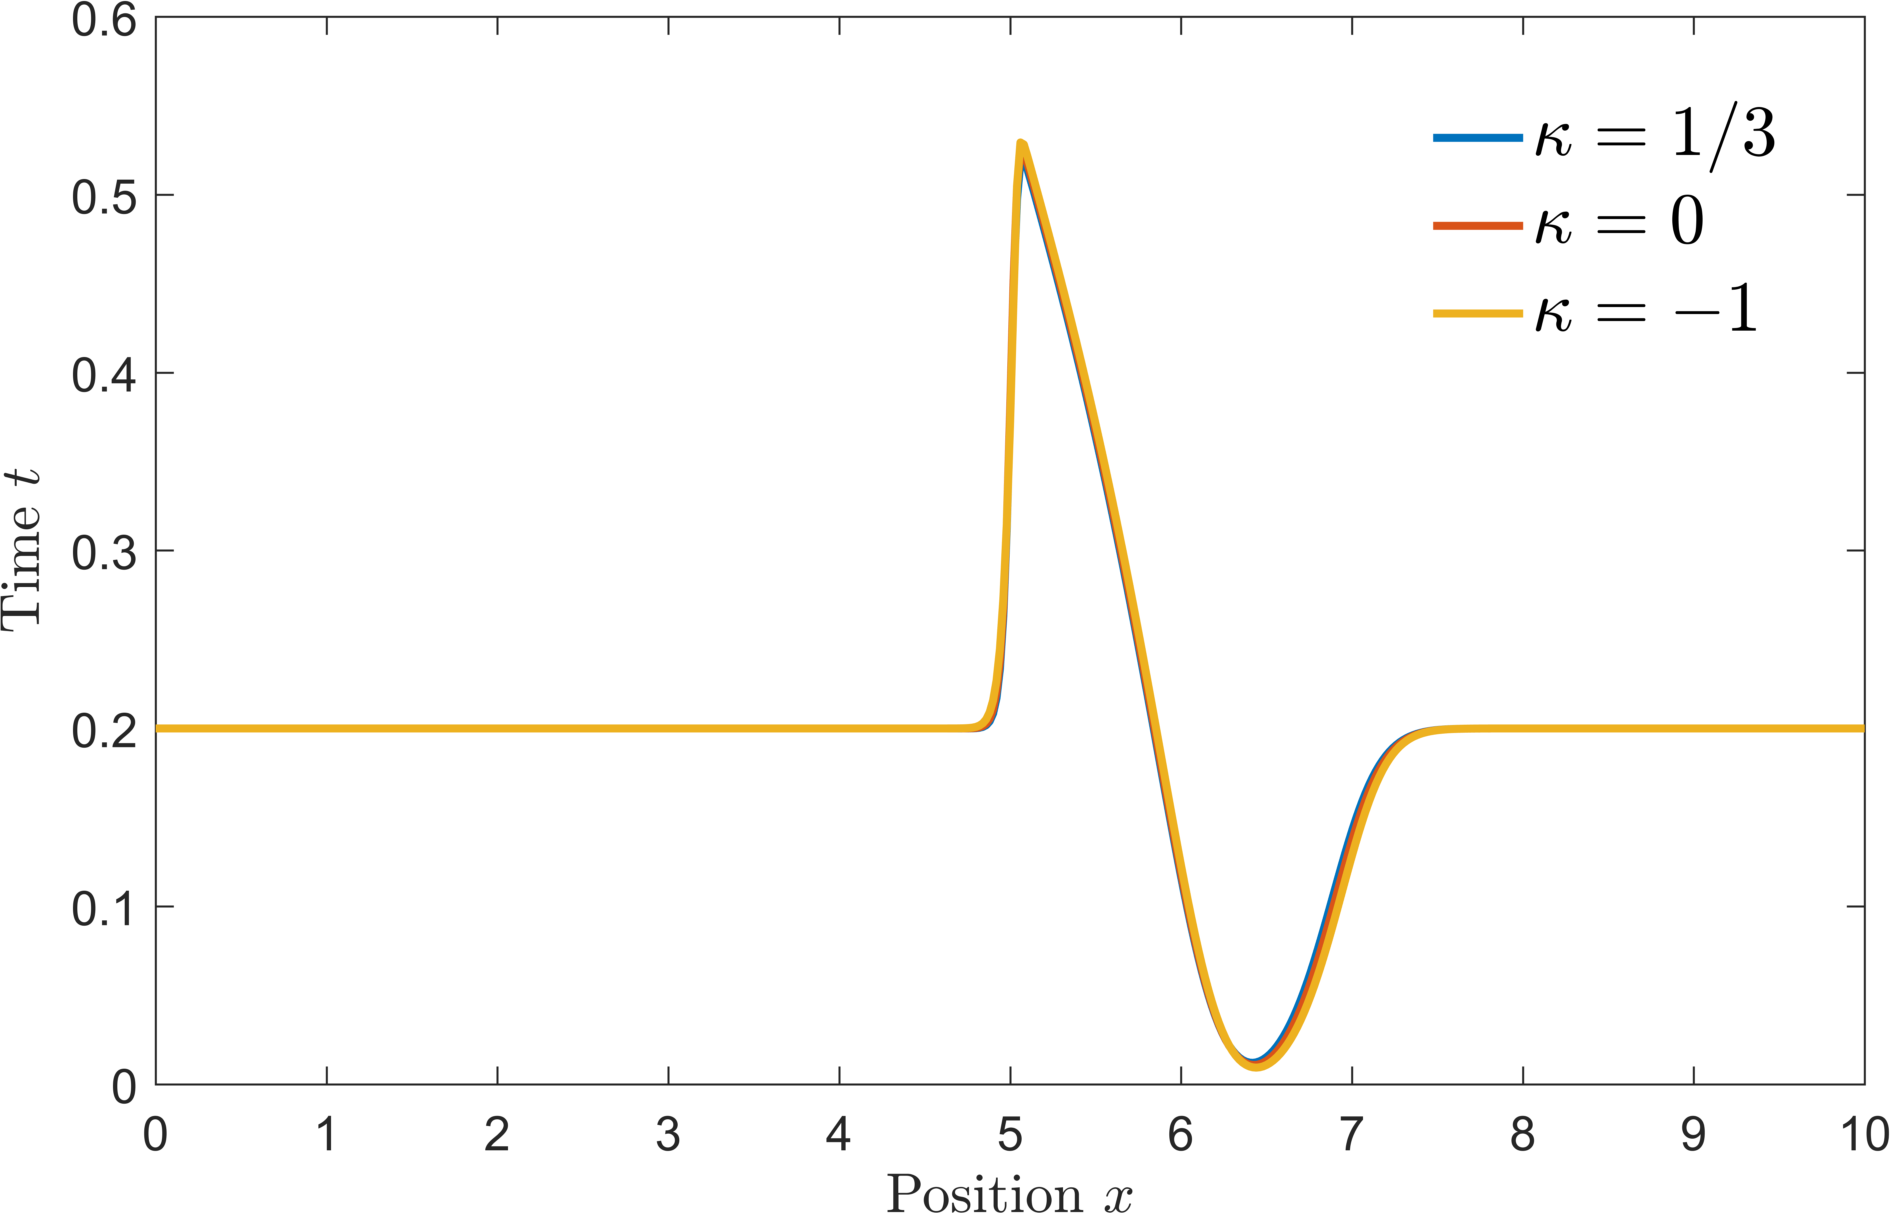
\includegraphics[width=\textwidth]{2a_light.png}
  \caption{Plot of $\rho(x,t=2)$ for light traffic, $\rho(0,t) = 0.2\rho_\mathrm{max}$, using multiple flux reconstruction schemes defined by the different $\kappa$ values.}
  \label{fig:2a_light}
\end{figure}

Qualitatively for the light traffic case we see no difference between the solutions produced by the second-order scheme in figure \ref{fig:2a_light} and the first-order scheme in figure \ref{fig:1b_light_surf}, and the value of $\kappa$ employed does not change the solution in any substaintial manner. The scheme appears to be stable with respect to changes in $\kappa$, quite a desirable quality. Perhaps in the light traffic case that was little need for a flux limiter function as the shockwave fans out rather quickly and the traffic density is not saturated for long. In particular, we notice no spurious oscillations, however we attribute this mainly to the robustness of MATLAB's \texttt{ode45} and its adaptive time stepping which appeared to step back in time once any spurious oscillations set in to adjust the time step accordingly such that the oscillations disappear. When they did set in, they mainly appeared at the traffic density peak.

\begin{figure}[h!]
  \centering
  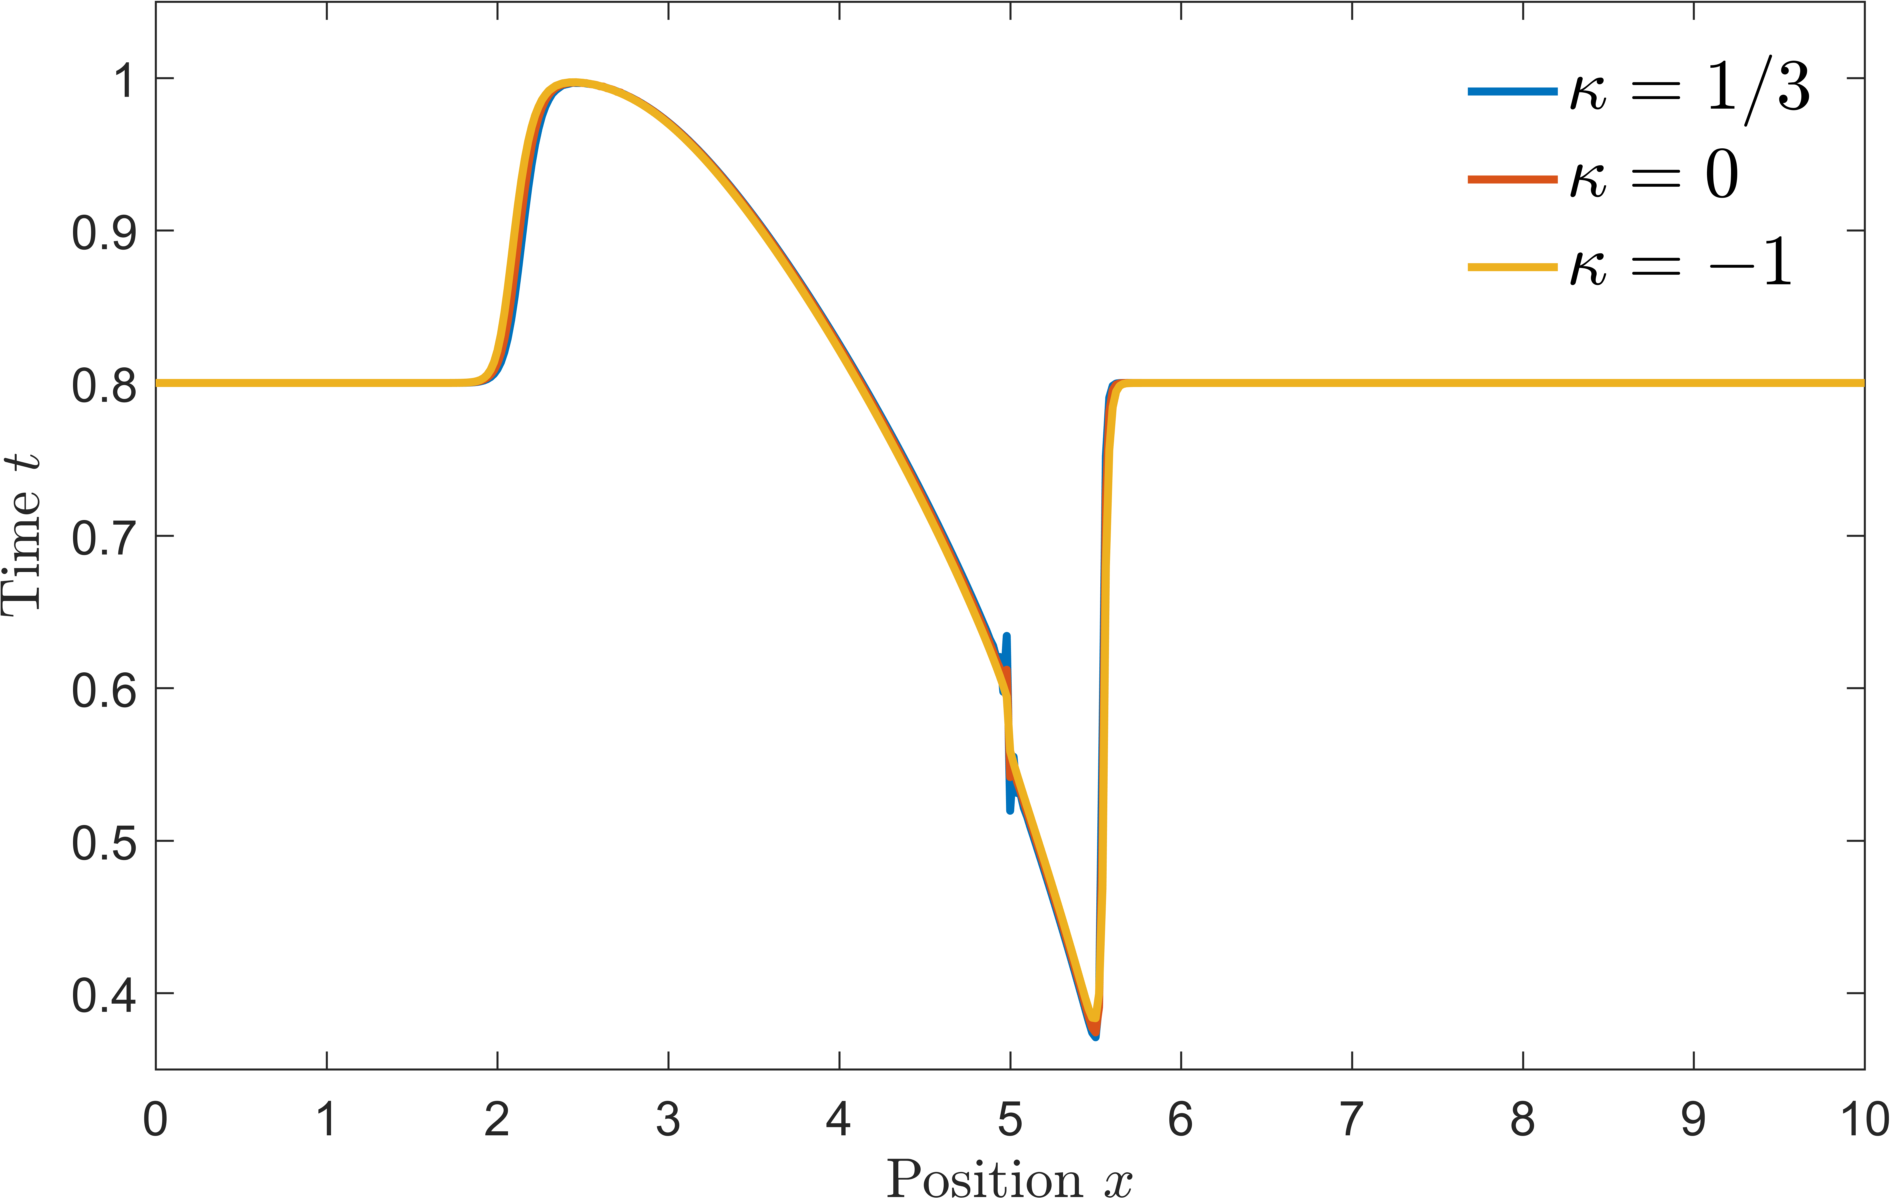
\includegraphics[width=\textwidth]{2a_heavy.png}
  \caption{Plot of $\rho(x,t=2)$ for heavy traffic, $\rho(0,t) = 0.8\rho_\mathrm{max}$, using multiple flux reconstruction schemes defined by the different $\kappa$ values, but with no flux limiter function in action.}
  \label{fig:2a_heavy}
\end{figure}

Likewise, for the heavy traffic case see no major differences between the solutions produced by the second-order scheme in figure \ref{fig:2a_heavy} and the first-order scheme in figure \ref{fig:1b_heavy_surf}. However, certain values of $\kappa$ now seem to introduce a small oscillation, which grows smaller with time, at the shockwave as it fans out. In particular, at $\kappa = -1$ no spurious oscillations of any kind are recognizable, however $\kappa = 0$ and $\kappa = 1/3$ produce increasingly larger oscillations. Again, some spurious oscillations do show up at the traffic density peak but \texttt{ode45} appears to do a fantastic job at adaptively time stepping to avoid them. Perhaps spurious oscillations are now are a larger problem as the shockwave persists for longer and slopes are much larger for the heavy traffic case, neccessitating the use of a flux limiter function.

\subsection{Flux reconstruction utilizing various limiter functions}
\begin{tcolorbox}
  \textit{Now employ the limited algorithm with the MinMod, Van Leer, and Superbee limiters. Again, utilize the same mesh size and time step as above, and all three values of $\kappa = -1$, $0$, and $1/3$. Describe the quality of these solutions, in particular how they compare with each other and with the solution obtained without limiters for the light traffic case. Again, it might be useful to look at the solutions at time t = 2.0 obtained with the different methods.}
\end{tcolorbox}

We will now introduce three different flux limiter functions $\phi(r)$ into the equations for the interface values \eqref{eq:kappa1} and \eqref{eq:kappa2} in an attempt to avoid extreme slope reconstructions and spurious oscillations.

The first we will consider is the minmod flux limiter function which takes the lower boundary of the total variation diminishing (TVD) region resulting in it being the \emph{most diffusive} flux limiter function. It can be written as
\begin{equation}
\phi_\mathrm{minmod}(r) = \max\left\{ 0, \min\left\{r,1\right\} \right\}
\end{equation}
while its counterpart, the superbee flux limiter function, is the \emph{least diffusive} limiter and can be written as 
\begin{equation}
\phi_\mathrm{superbee}(r) = \max \left\{ 0, \min\left\{2r,1\right\}, \min\left\{r,2\right\} \right\}
\end{equation}
and represents the upper boundary of the TVD region. The third flux limiter function we will consider is the van Leer flux function can be written as
\begin{equation}
\phi_\mathrm{van Leer}(r) = \frac{r + |r|}{1 + |r|}
\end{equation}
and takes on a value in between the minmod and superbee limiters. It is second-order accurate when the solution is smooth, and downgrades to upwind or first-order accurate at discontinuities.

Trying out each flux limiter function for each value of $\kappa \in {-1,0,1/3}$. We plot the traffic density at $t=2$ for each of the nine cases in figure \ref{fig:2b_all}.

\begin{figure}[h!]
  \centering
  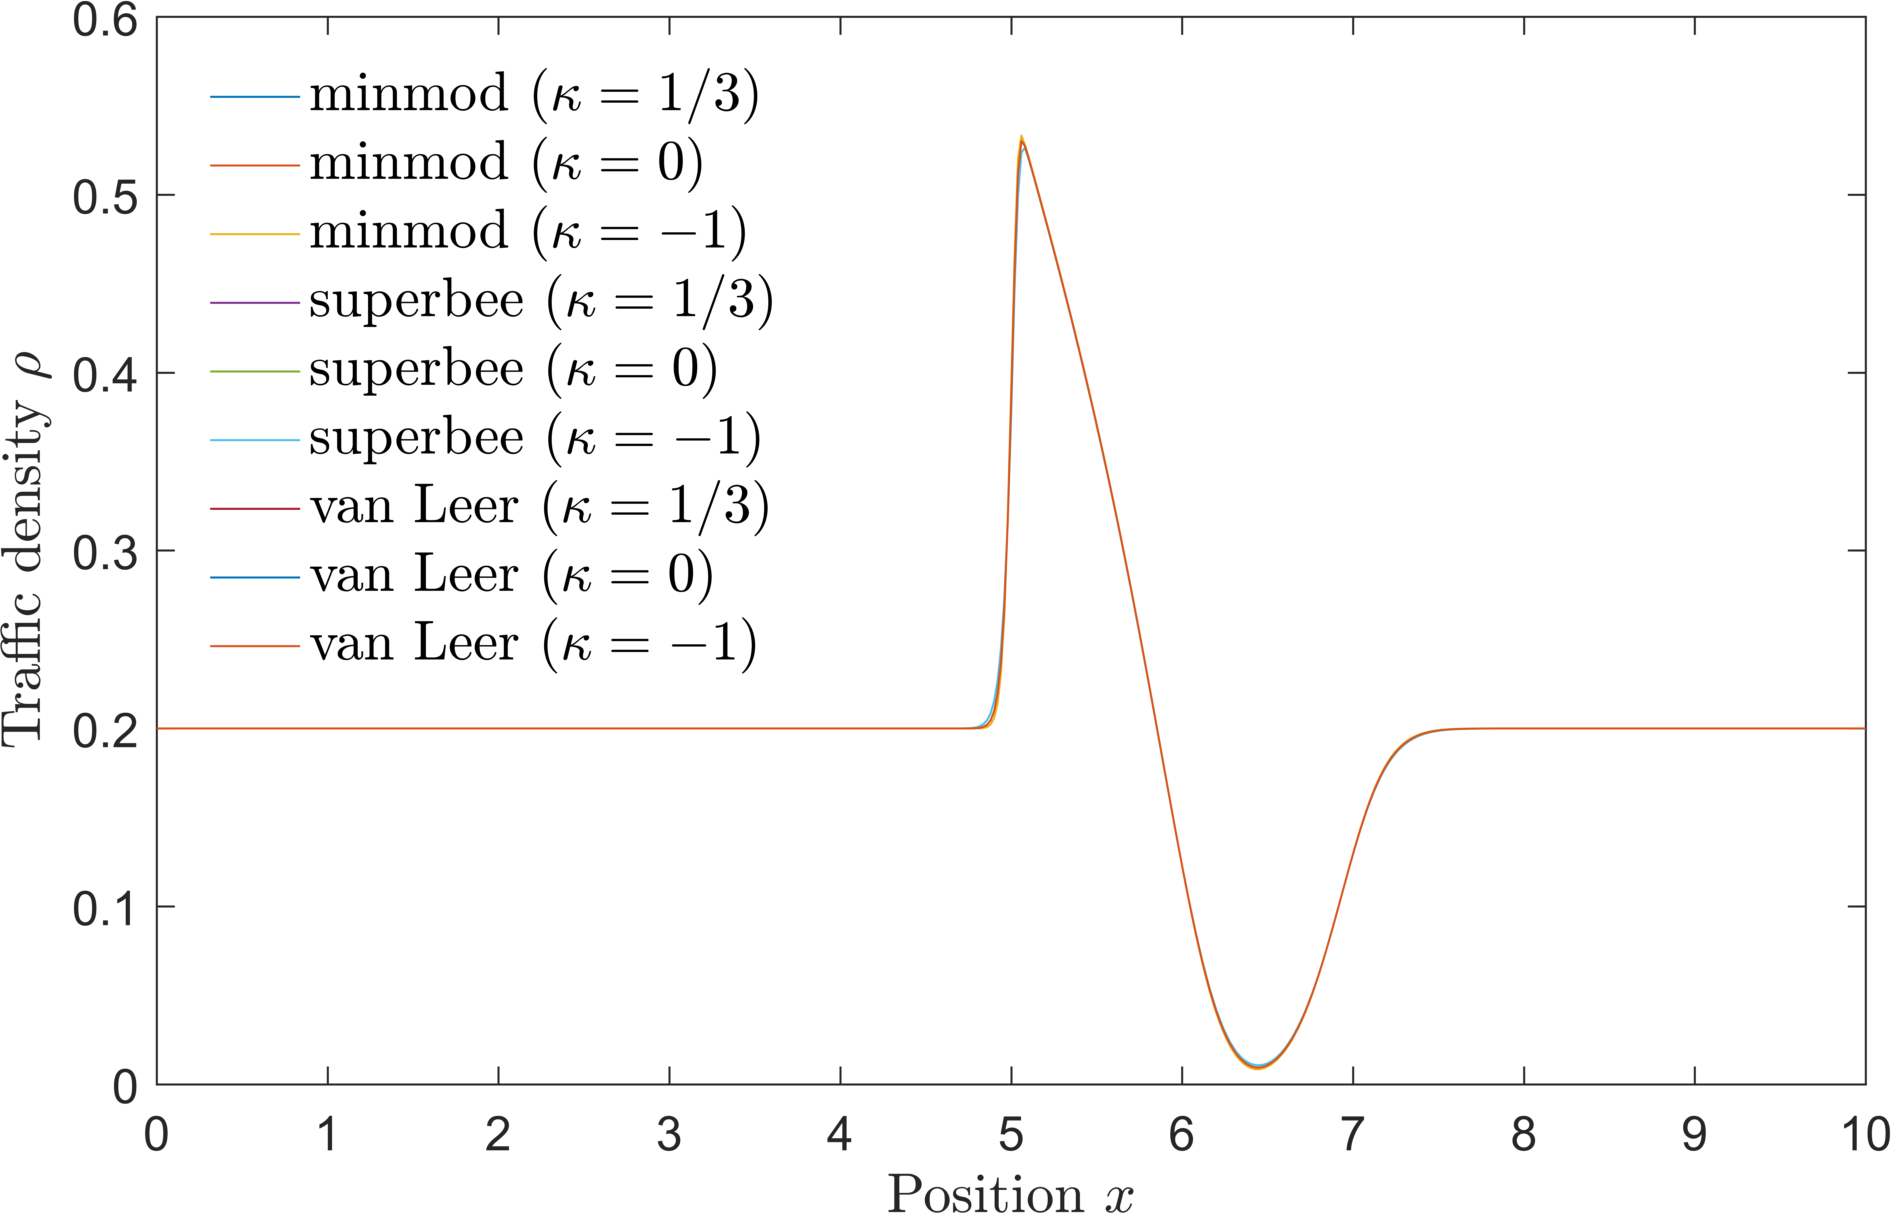
\includegraphics[width=\textwidth]{2b_all.png}
  \caption{Plot of $\rho(x,t=2)$ for light traffic, $\rho(0,t) = 0.2\rho_\mathrm{max}$, using multiple flux limiter schemes (minmod, Superbee, and van Leer) and multiple flux reconstruction schemes defined by the different $\kappa$ values.}
  \label{fig:2b_all}
\end{figure}

We immediately notice almost no difference in any of the solutions produced as they overlap almost perfectly except for tiny numerical differences. They agree almost exactly with the solution produced using no flux limiter function in figure \ref{fig:2a_light}. We previously suspected that the light traffic case did not suffer much from extreme slope reconstructions, however, what is surprising is the degree to which all the solutions agree. Perhaps there would be more variability had I implemented my own fourth-order Runge-Kutta time integration scheme but for serious applications, no one would implement their own \texttt{ode45} and reinvent the wheel. Our solution, especially for the light traffic case, appears to be rather well-behaved compared to other nonlinear partial differetial equations exhibiting shockwaves so perhaps these flux limiter functions find much more utility when applied to other problems or to higher-dimensional problems. I would have looked at the heavy traffic case but it was not required for this problem set.

\section{Multi-lane problems}
The first thing we will do here is rewrite the lane-switching source term \eqref{eq:source} to be more friendly to compute. We will assume we have $n$ lanes indexed by $\ell=1,2,\dots,n$. Drivers can only switch in from neighbouring lanes due to the $|k-\ell|=1$ constraint and only into lanes with lower traffic densities, so $s^{(1)} = \alpha \left( \rho^{(2)} - \rho^{(1)} \right)$ and $s^{(n)} = \alpha \left( \rho^{(n-1)} - \rho^{(n)} \right)$, otherwise $s^{(\ell)} = \alpha \left( \rho^{(\ell+1)} - 2\rho^{(\ell)} + \rho^{(\ell-1)} \right)$ for $1 < \ell < n$. Thus the source term can be written as 
\begin{equation} \label{eq:sourceEasy}
s^{(\ell)} = \sumop_{\substack{|k-\ell|=1 \\ 1 \le k,\ell \le n}} \alpha \left( \rho^{(k)} - \rho^{(\ell)} \right) = \alpha
\begin{cases}
  \rho^{(2)} - \rho^{(1)},& \text{if } \ell = 1 \\
  \rho^{(\ell+1)} - 2\rho^{(\ell)} + \rho^{(\ell-1)},& \text{if } 1 < \ell < n \\
  \rho^{(n-1)} - \rho^{(n)},& \text{if } \ell = n
\end{cases}
\end{equation}

\subsection{Multi-lane traffic simulation with an impulsive source term}
\begin{tcolorbox}
  \textit{Ethan Hunter reasons that traffic behaves like a living organism and takes the example when a driver brakes abruptly on a highway. Effectively the abrupt breaking can be modeled as an impulsive source term $S$ at $t = 0$ at $x = 5$ in some initial traffic $\rho_\mathrm{init}$ where $\alpha = 0.1$. Find a initial condition or relationship between $S$ and $\rho_\mathrm{init}$ such that a shock wave forms later in time for the single, double and a triple lane case.}
\end{tcolorbox}

In modeling multiple lanes we simply solve the conservative scalar law \eqref{eq:conservationLaw} for each lane $\ell$ using the $\kappa$-reconstructions given by \eqref{eq:kappa1} and \eqref{eq:kappa2} to compute the cell interface values with $\kappa=-1$ as it seemed to be the most stable in figure \ref{fig:2a_heavy}. The superbee flux limiter is employed because I think, probably erranously, that it's \emph{least diffusive} nature might help in observing the sharp shockwaves. 

Ideally we would want to model the sudden braking by Dirac delta functions, or distributions to be proper, such that $S(x,t) = \delta(t)\delta(x-x_0)$. However, introducing infinities numerically will be disastrous and so we will simply add a finite-valued impulse source term at the first time step $n=1$ and at $x=5$ or cell $i=N/2$. Letting $S_0 \in \mathbb{R}$ be the magnitude of the impulse, we will use the discrete version of the Dirac delta function, the Kronecker delta tensor $\delta_{ij}$ and write $S(x,t) = S_0\delta_{n1}\delta_{i,\frac{N}{2}}$. The value of $S_0$ must be continously adjusted for each numerical experiment to avoid cases where $\rho(x,t) > \rho_\mathrm{max}$ and to avoid creating cars out of thin air. However, the traffic dynamics seem to qualitatively make sense even with a bit of non-conservative behavior. To keep the scheme conservative, we could apply a negative forcing term $S_{-}(x,t) = -S_0\delta_{n1}\delta_{i,\frac{N}{2}+1}$ to the cell to the right of the one forced by $+S(x,t)$ to simulate the decreasing density of cars ahead of the sudden braker.

For the 1-lane case, it seems that any value of $\rho_\mathrm{init}$ and $S$ produces a shockwave. Like in the case of the simulated car accident, the traffic density wave propagates backwards for high values of $\rho_\mathrm{init}$ and forwards for low $\rho_\mathrm{init}$. The higher the traffic density, the longer the shockwave lives.

For the 2 and 3-lane case, it appears that the shockwave decays more rapidly as cars are allowed to change lanes. However, for $\alpha=0.1$ is it not that much more rapid as the lane switching source term is proportional to the difference in density, which tends to be quite small over most of the domain, then is multiplied by $\alpha$. Figure \ref{fig:q3a_3lanes} shows an example solution for $n=3$ lanes. The shockwave has already began to decay on lane 2, helped by 

\begin{figure}[h!]
  \centering
  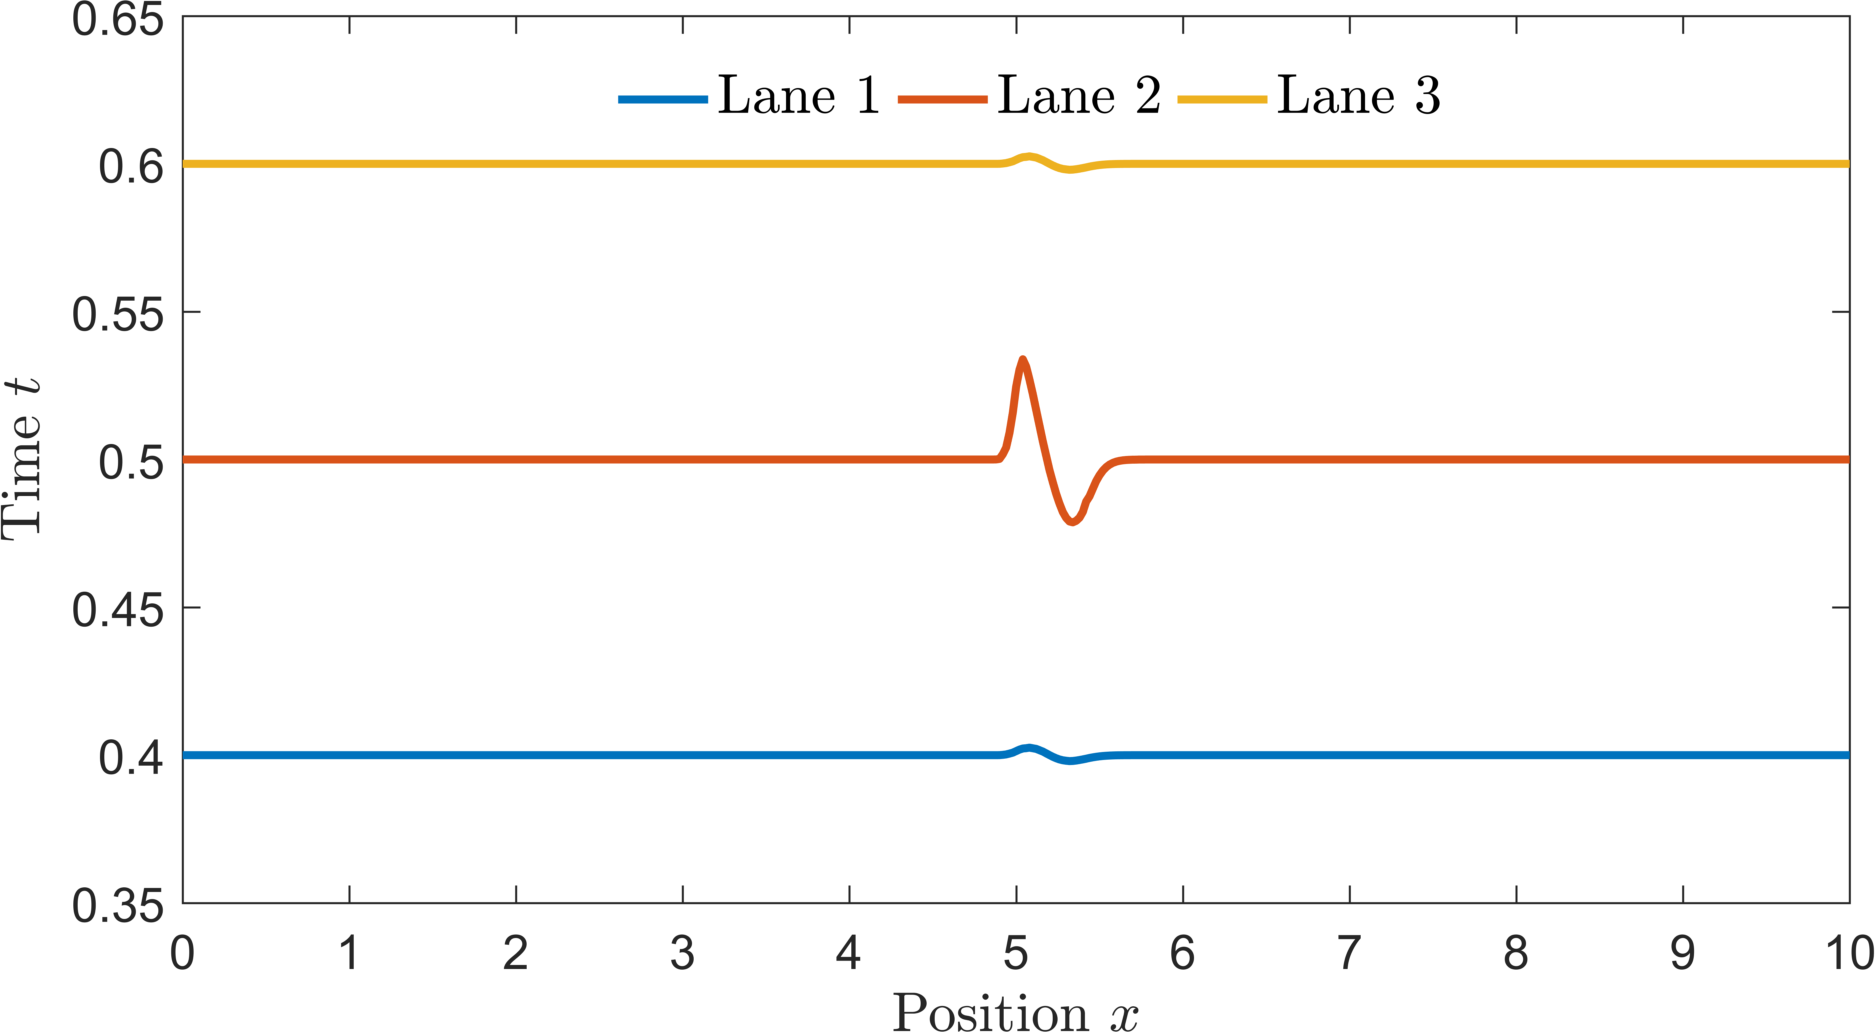
\includegraphics[width=\textwidth]{q3a_3lanes.png}
  \caption{Plot of $\rho(x,t=1.6)$ for intermediate traffic, $\rho_\mathrm{init} = 0.5\rho_\mathrm{max}$ for each lane, using $\kappa=-1$ with the Superbee flux limiter scheme. Lane 1 was offset by $-0.1$ and lane 3 was offset by $+0.1$.}
  \label{fig:q3a_3lanes}
\end{figure}

Physically, however, I would differentiate between a large shockwave actually representing a buildup of traffic and a small shockwave representing one car suddenly braking. Furthermore, I would expect that $\rho_\mathrm{init}$ cannot be not too low or too high, possibly even the existance of two critical values between which a shockwave is formed in the middle lane. If $\rho_\mathrm{init}$ is too low then there is very little traffic density to respond appreciably to the sudden braking, that is, there are no cars behind the braking car so no one else slows down and business continues on as usual. In this case, I suppose the shockwave decays rapidly. If $\rho_\mathrm{init}$ is too high, then the cars are already travelling quite slowly so a sudden braking just slows the cars down just a little and they continue on afterwards. However, in the intermediate case when cars are travelling quite quickly and traffic density is intermediate, a sudden braking could cause the one or two cars behind you to slow down substantially which could result in a propagating shockwave if there are enough cars behind the sudden braker in rather close proximity.

\subsection{Multi-lane simulation with an accident and time-delayed switching term}
Unfortunately I watched too much Netflix over the long weekend (was worth it, would recommend American Vandal) and did not leave myself enough time to attempt this question.

\end{document}